In this section we will present the different concepts and paradigms that will be explored throughout this thesis.
Specifically, we will detail the Software Defined Networking paradigm, and the network virtualization techniques that have emerged from it.

\subsection{Software Defined Networking}

Traditional networks are complex and difficult to operate~\cite{complexnetworks}, due to their heterogeneity and lack of interoperability. The network administrator is often tasked to configure each network element individually, and has to either do it manually or use low-level vendor specific scripts to deploy the configuration. The impossibility to aggregate these tasks into a unified flow becomes more and more problematic as network infrastructures grow, especially for Cloud Providers.

To overcome these aspects, a new networking paradigm has been proposed, namely Software Defined Networking (SDN).
The SDN paradigm consists in decoupling the control plane and the data plane.
The control plane is in charge of deciding how the network traffic should be processed upon entering the SDN infrastructure.
This task is performed by a centralized component called ''SDN controller`` and lies between end users and the physical infrastructure (see Figure~\ref{fig:SDN-archi}. Instead of considering network traffic as a sequence of packets, SDN aggregate packets into flows that are described by a match pattern (filter) and every packet belonging to the flow will be processed identically. Figure~\ref{fig:matching-fields} summarizes the different header fields a flow can be matched against.

\begin{figure}[htbp]
\centering





\tikzset{every picture/.style={line width=0.75pt}} %set default line width to 0.75pt        

\begin{tikzpicture}[x=0.75pt,y=0.75pt,yscale=-1,xscale=1]
%uncomment if require: \path (0,777); %set diagram left start at 0, and has height of 777

%Straight Lines [id:da17115450592431847] 
\draw [color={rgb, 255:red, 208; green, 2; blue, 27 }  ,draw opacity=1 ][line width=2.25]  [dash pattern={on 6.75pt off 4.5pt}]  (293,217.9) -- (235,268.86) ;


%Shape: Cloud [id:dp2708604447913189] 
\draw   (157.06,281.41) .. controls (158.39,271.23) and (173.56,262.61) .. (196.13,259.2) .. controls (218.71,255.81) and (244.73,258.22) .. (263.15,265.44) .. controls (273.16,260.49) and (288.45,257.95) .. (304.4,258.6) .. controls (320.34,259.25) and (335.07,263.01) .. (344.13,268.73) .. controls (352.8,264.2) and (366.72,262.01) .. (380.94,262.94) .. controls (395.17,263.86) and (407.68,267.78) .. (414.04,273.29) .. controls (427.91,268.98) and (446.99,268.56) .. (463.02,272.21) .. controls (479.05,275.86) and (489.15,282.93) .. (488.96,290.36) .. controls (502.1,293.38) and (511.8,298.57) .. (515.56,304.58) .. controls (519.32,310.6) and (516.76,316.85) .. (508.56,321.71) .. controls (518.81,330.49) and (517.45,340.61) .. (505.02,348.29) .. controls (492.58,355.97) and (470.92,360.06) .. (448.13,359.03) .. controls (444.23,367.06) and (430.13,373.31) .. (411.24,375.38) .. controls (392.36,377.46) and (371.65,375.02) .. (357.09,369.02) .. controls (345.58,377.91) and (322.46,382.91) .. (297.73,381.85) .. controls (273,380.8) and (251.1,373.88) .. (241.48,364.09) .. controls (223.01,366.47) and (202.59,365.56) .. (184.83,361.57) .. controls (167.07,357.58) and (153.47,350.85) .. (147.09,342.89) .. controls (129.79,341.92) and (115.12,336.58) .. (110.35,329.5) .. controls (105.58,322.43) and (111.73,315.13) .. (125.75,311.24) .. controls (112.37,305.98) and (108.05,297.88) .. (115.05,291.17) .. controls (122.06,284.47) and (138.8,280.67) .. (156.54,281.76) ; \draw   (125.76,311.24) .. controls (132.08,313.72) and (139.94,315.38) .. (148.29,315.98)(147.1,342.89) .. controls (150.71,343.09) and (154.35,343.1) .. (157.91,342.9)(241.48,364.09) .. controls (239.7,362.28) and (238.38,360.41) .. (237.55,358.51)(357.09,369.02) .. controls (359.19,367.4) and (360.87,365.67) .. (362.09,363.88)(448.12,359.03) .. controls (452.27,350.48) and (444.14,341.4) .. (427.23,335.68)(508.56,321.71) .. controls (504.18,324.31) and (498.37,326.41) .. (491.58,327.85)(488.96,290.36) .. controls (488.92,291.59) and (488.6,292.81) .. (488.01,294)(414.04,273.29) .. controls (410.58,274.36) and (407.55,275.65) .. (405.02,277.11)(344.13,268.73) .. controls (342.05,269.82) and (340.31,271.02) .. (338.96,272.3)(263.15,265.44) .. controls (267.04,266.96) and (270.51,268.67) .. (273.47,270.52)(157.06,281.41) .. controls (156.87,282.82) and (156.95,284.23) .. (157.3,285.64) ;
%Straight Lines [id:da33177785199586485] 
\draw    (191,329.03) -- (227,279.5) ;


%Straight Lines [id:da150748682776351] 
\draw    (206,327.12) -- (405,281.88) ;


%Straight Lines [id:da9129920016149438] 
\draw    (227,279.5) -- (410,279.5) ;


%Straight Lines [id:da09977910639670284] 
\draw    (464,336.65) -- (410,279.5) ;


%Straight Lines [id:da1789459372776585] 
\draw    (464,336.65) -- (197,329.03) ;


%Rounded Rect [id:dp48669800314404355] 
\draw  [fill={rgb, 255:red, 242; green, 179; blue, 186 }  ,fill opacity=1 ] (91.53,163.68) .. controls (91.53,161.58) and (93.24,159.87) .. (95.34,159.87) -- (535.19,159.87) .. controls (537.29,159.87) and (539,161.58) .. (539,163.68) -- (539,175.11) .. controls (539,177.22) and (537.29,178.92) .. (535.19,178.92) -- (95.34,178.92) .. controls (93.24,178.92) and (91.53,177.22) .. (91.53,175.11) -- cycle ;

%Rounded Rect [id:dp7182041839424143] 
\draw  [fill={rgb, 255:red, 255; green, 255; blue, 255 }  ,fill opacity=1 ] (91.53,211.31) .. controls (91.53,209.2) and (93.24,207.5) .. (95.34,207.5) -- (534.19,207.5) .. controls (536.29,207.5) and (538,209.2) .. (538,211.31) -- (538,222.74) .. controls (538,224.84) and (536.29,226.55) .. (534.19,226.55) -- (95.34,226.55) .. controls (93.24,226.55) and (91.53,224.84) .. (91.53,222.74) -- cycle ;

%Rounded Rect [id:dp21600182347401065] 
\draw  [fill={rgb, 255:red, 255; green, 255; blue, 255 }  ,fill opacity=1 ] (91.53,116.05) .. controls (91.53,113.95) and (93.24,112.24) .. (95.34,112.24) -- (534.72,112.24) .. controls (536.83,112.24) and (538.53,113.95) .. (538.53,116.05) -- (538.53,127.48) .. controls (538.53,129.59) and (536.83,131.29) .. (534.72,131.29) -- (95.34,131.29) .. controls (93.24,131.29) and (91.53,129.59) .. (91.53,127.48) -- cycle ;

%Straight Lines [id:da7180441165592505] 
\draw [color={rgb, 255:red, 208; green, 2; blue, 27 }  ,draw opacity=1 ][line width=2.25]  [dash pattern={on 6.75pt off 4.5pt}]  (313,227.42) -- (393,272.67) ;


%Up Down Arrow [id:dp6954251131148171] 
\draw  [color={rgb, 255:red, 0; green, 0; blue, 0 }  ,draw opacity=1 ][fill={rgb, 255:red, 126; green, 126; blue, 126 }  ,fill opacity=1 ][line width=2.25]  (278,138.24) -- (313,131.21) -- (348,138.24) -- (330.5,138.24) -- (330.5,152.29) -- (348,152.29) -- (313,159.32) -- (278,152.29) -- (295.5,152.29) -- (295.5,138.24) -- cycle ;
%Up Down Arrow [id:dp1361930975498693] 
\draw  [color={rgb, 255:red, 0; green, 0; blue, 0 }  ,draw opacity=1 ][fill={rgb, 255:red, 126; green, 126; blue, 126 }  ,fill opacity=1 ][line width=2.25]  (278,186.82) -- (313,179.8) -- (348,186.82) -- (330.5,186.82) -- (330.5,200.87) -- (348,200.87) -- (313,207.9) -- (278,200.87) -- (295.5,200.87) -- (295.5,186.82) -- cycle ;
%Rounded Rect [id:dp6282943511852553] 
\draw  [fill={rgb, 255:red, 115; green, 241; blue, 241 }  ,fill opacity=1 ] (91.53,90.81) .. controls (91.53,88.71) and (93.24,87) .. (95.34,87) -- (535.19,87) .. controls (537.29,87) and (539,88.71) .. (539,90.81) -- (539,102.24) .. controls (539,104.35) and (537.29,106.05) .. (535.19,106.05) -- (95.34,106.05) .. controls (93.24,106.05) and (91.53,104.35) .. (91.53,102.24) -- cycle ;

%Image [id:dp7612823546286228] 
\draw (220.5,288.25) node  {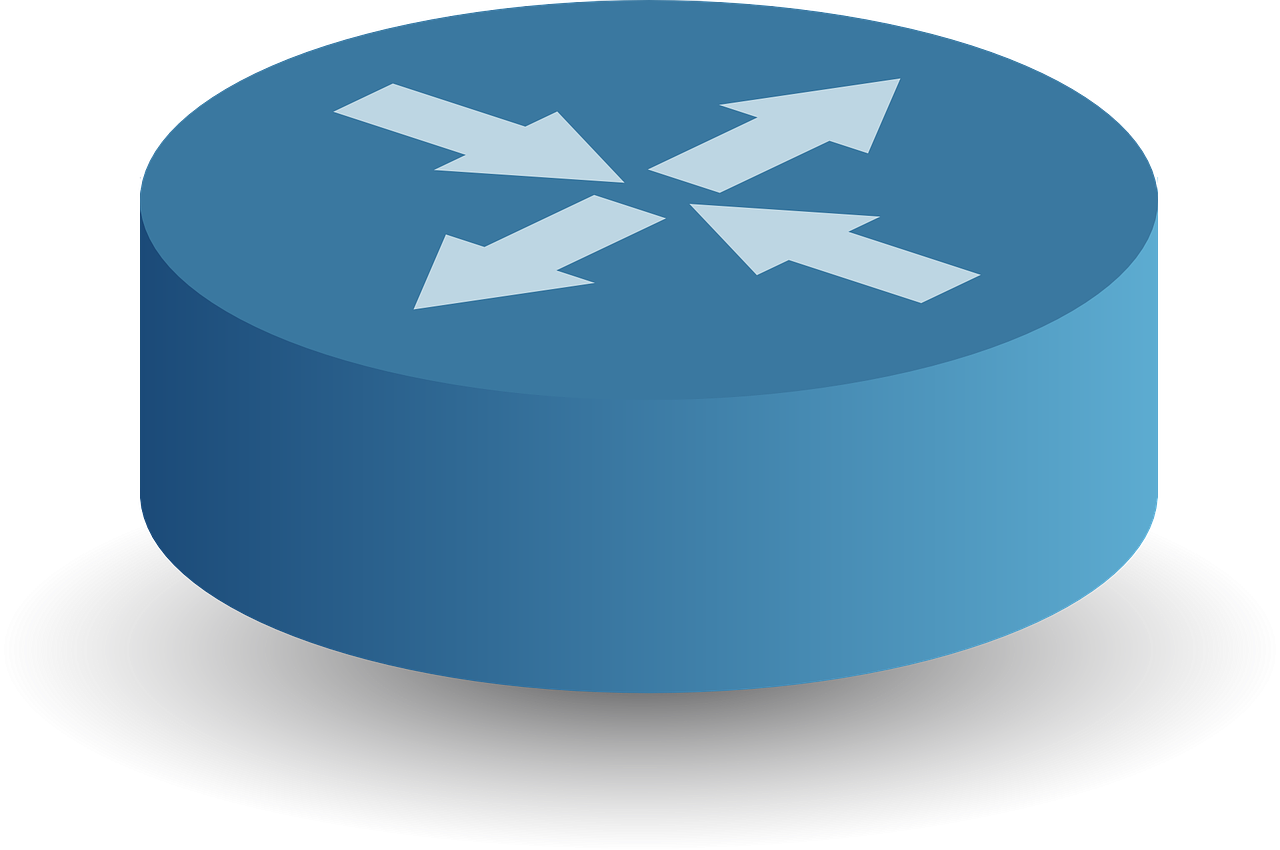
\includegraphics[width=42.75pt,height=39.38pt]{figures/router-29825_1280.png}};
%Image [id:dp3067390553920406] 
\draw (194.5,340.25) node  {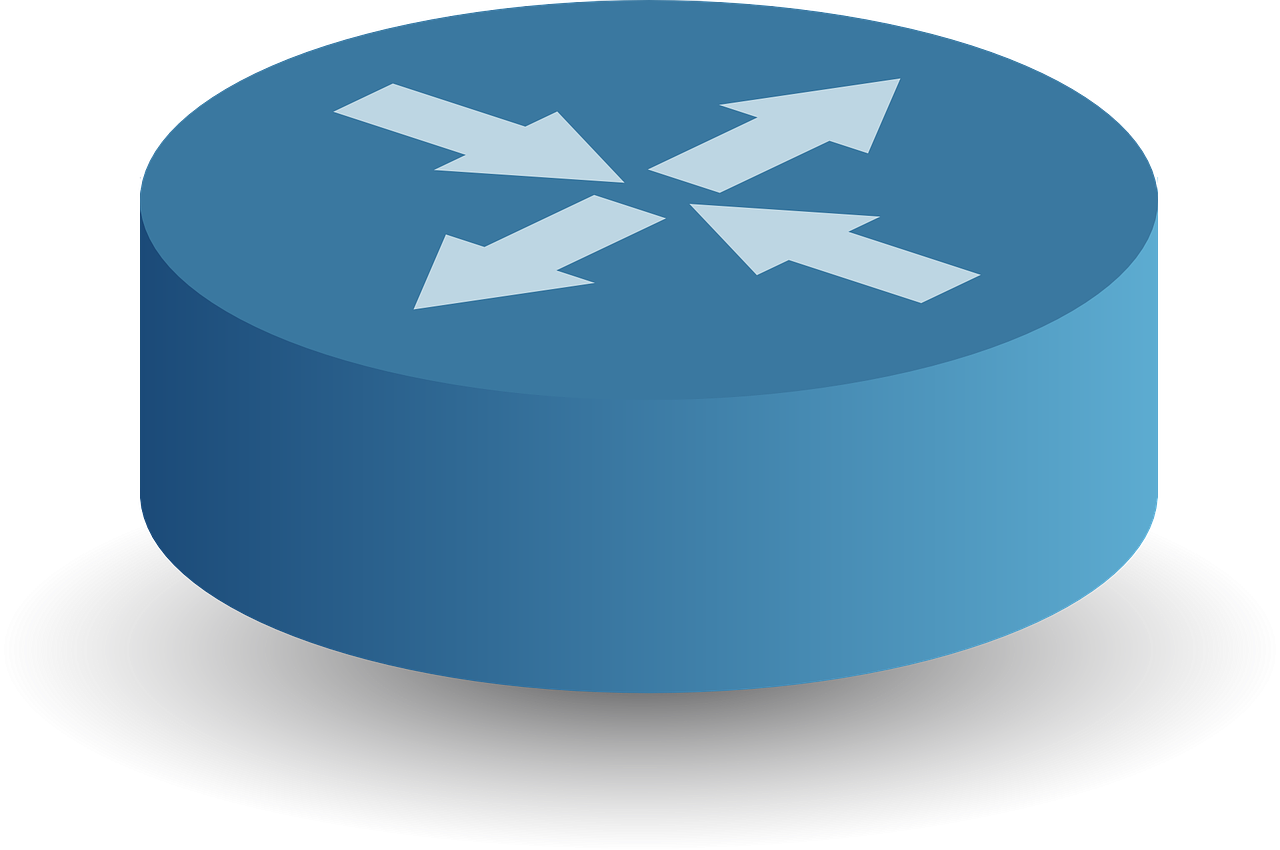
\includegraphics[width=42.75pt,height=39.38pt]{figures/router-29825_1280.png}};
%Image [id:dp24035408652285217] 
\draw (454.5,340.25) node  {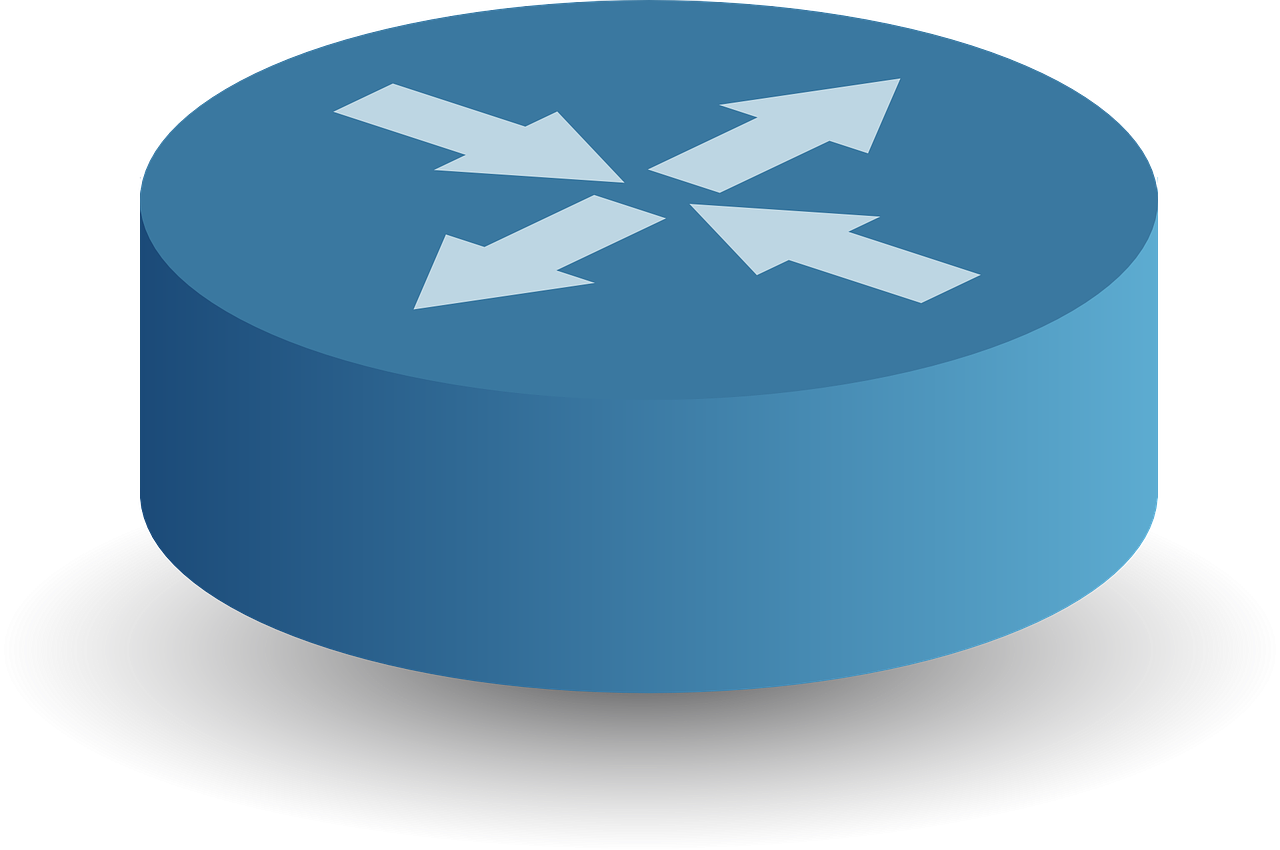
\includegraphics[width=42.75pt,height=39.38pt]{figures/router-29825_1280.png}};
%Image [id:dp7735606932716308] 
\draw (404.5,296.25) node  {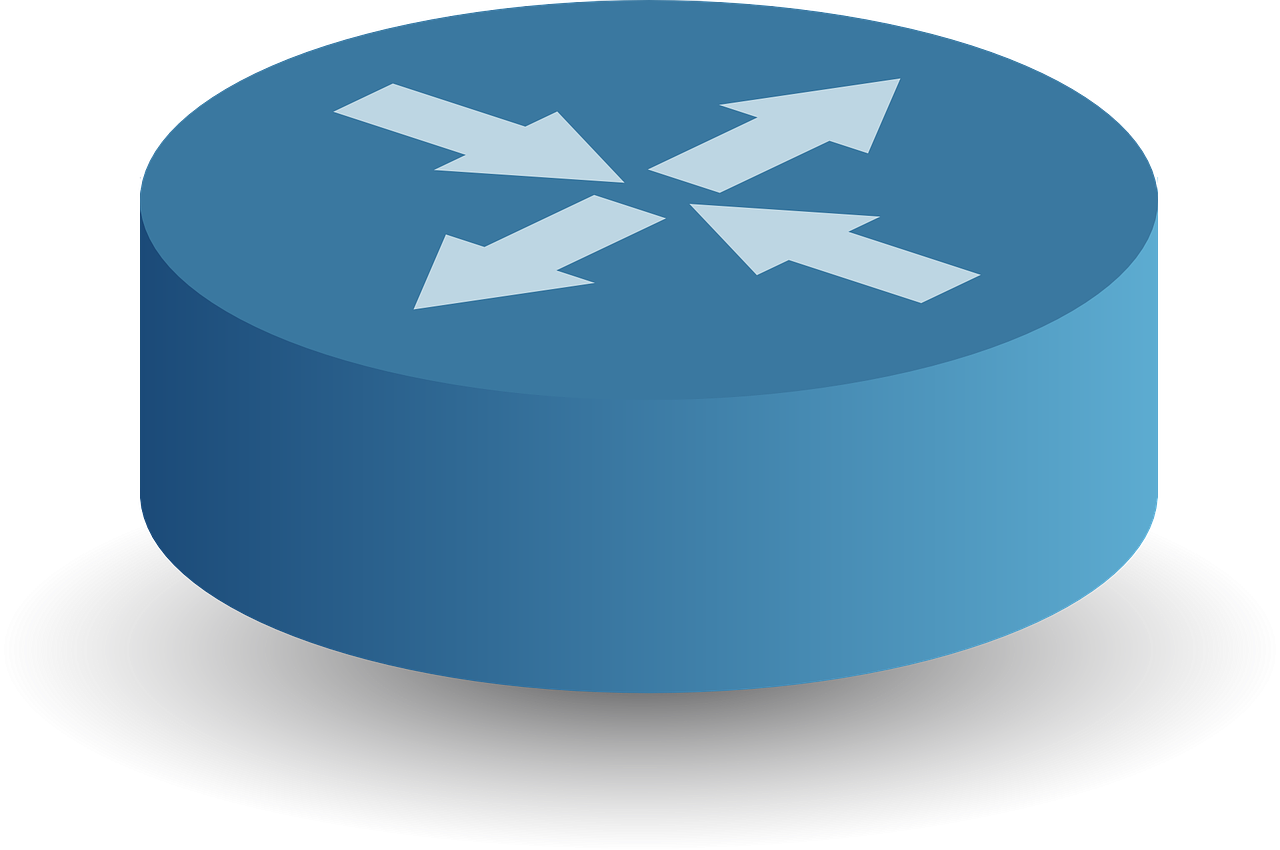
\includegraphics[width=42.75pt,height=39.38pt]{figures/router-29825_1280.png}};

% Text Node
\draw (315.27,96.53) node  [align=left] {SDN Applications};
% Text Node
\draw (315.03,121.77) node  [align=left] {Northbound API};
% Text Node
\draw (314.77,217.02) node  [align=left] {Southbound API};
% Text Node
\draw (315.27,169.4) node  [align=left] {SDN Controller};


\end{tikzpicture}

\caption{Software Defined Networking Architecture}
\label{fig:SDN-archi}
\end{figure}

The programmability of the network has given developers a lot of flexibility to design new services and network applications that will run on top of the SDN controller.
For instance, a load balancing application can prioritize how the customer's traffic should be processed, following specific Quality of Service (QoS) requirements.
Another example is a firewall that may decide to drop all the packet from a specific source because of a Denial of Service (DoS) attack.
Applications can interact with the SDN controller via the Northbound API.
Usually, SDN controllers implement a REST API for these interactions~\cite{onos-Berde2014a,opendaylight,floodlight}.
OpenFlow~\cite{Openflow-McKeown2008} is considered the standard implementation of the SDN paradigm, with numerous vendors including it in their products.
OpenFlow provides an southbound interface to communicate with switches and to install specific configurations using a match-action formalism.

\begin{figure}[h]
    \centering
    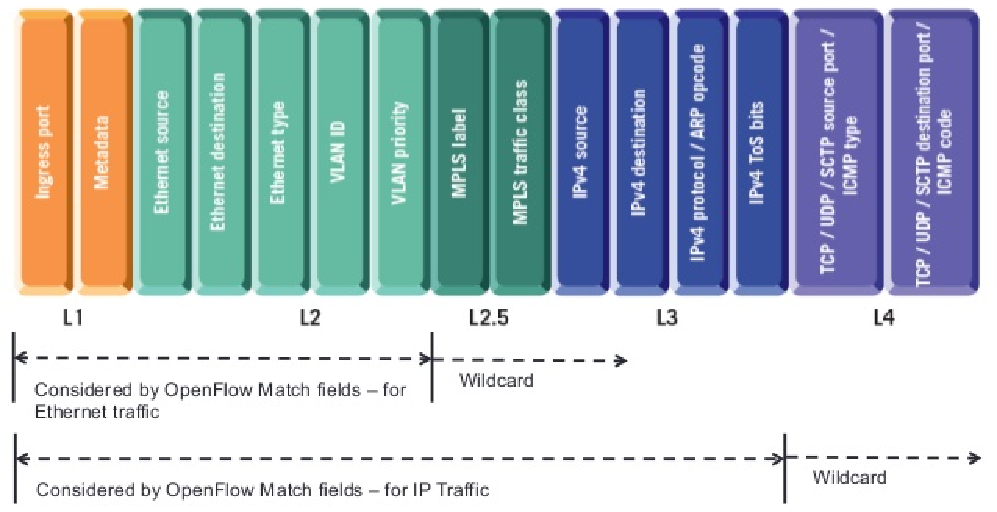
\includegraphics[scale=0.7]{figures/openflow-matchfields.pdf}
    \caption{OpenFlow matching fields~\cite{openflow-matchfields}}
    \label{fig:matching-fields}
\end{figure}

\subsection{Network Virtualization using SDN}
\label{def:netvirt}

For decades hypervisors have enabled the sharing of physical resources among several virtual machines.
Multiple users can run their own operating system simultaneously over a single physical machine.
VLANs, MPLS and VRF only provided limited virtualization for the network resource. The emergence of SDN and its flexibility for the design of network application has been leveraged to give network a reliable virtualization solution.

Figure~\ref{fig:virt-archi} illustrate the differences between a classic SDN environment and a virtualization infrastructure. In part (a), different applications will be deployed on the SDN controller and will impact the whole physical network.
In part (b), the network hypervisor abstracts the view of the physical infrastructure into virtual networks to the end users (also referred to as tenants).
Each tenant will be able to deploy its applications on his own virtual network, that will in turn only impact the physical resources associated to it.

\begin{figure}[ht]
    \centering
    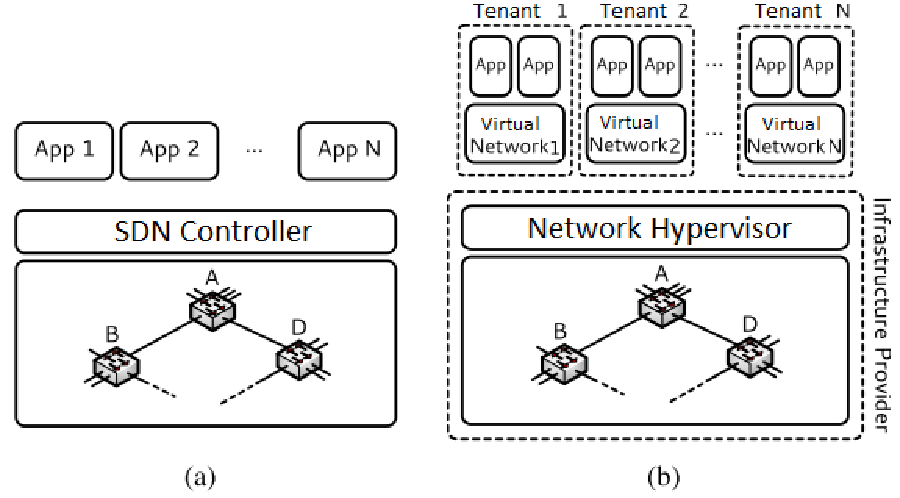
\includegraphics[scale=0.9]{figures/virt-archi.pdf}
    \caption{SDN infrastructure (a) vs. Virtualization infrastructure (b) from VeRTIGO~\cite{VeRTIGO-Corin2012a}}
    \label{fig:virt-archi}
\end{figure}


The process of mapping a virtual network with its underlying resources is referred to as the Virtual Network Embedding, and is illustrated in Figure~\ref{fig:VNE}.
The hypervisor is in charge to provide isolation between tenants, preventing them to interact with other tenants' virtual networks. Isolation covers either the resources allocated to tenants, such as bandwidth, switch CPU or flow tables memory, but it also includes the topology itself so a tenant cannot manipulate traffic that does not belong to him.

Two main information are used by tenants of the virtualization infrastructure, the address space and the flowspace.\\
\textbf{The address space} is the set of IP addresses that a tenant can assign to the hosts in his virtual network.\\
\textbf{The flowspace} is the set of header parameters the tenant can use when deploying flow rules to configure his virtual network (see Figure~\ref{fig:matching-fields}). The hypervisor may restrict the use of certain headers because the virtualization already uses them as internal identifiers.

Presenting a virtual network to the tenant can be done in two different ways, either by slicing the physical infrastructure or by abstracting it.\\
\textbf{A slice} is the set of resources allocated to a virtual network.
Slicing the physical infrastructure consists in presenting the tenant with only a smaller part of the infrastructure while hiding the rest of the network equipments.
The hypervisor gives tenants a direct access to the network nodes composing the slice, and the flow rules installed by the tenant will be rewritten to match the flow space he has been allocated.\\
The term slice is also found in the literrature to describe the subdivision of a single physical resource. For instance, a slice can be a subdivision of a physical node corresponding to a specific tenant.\\
\textbf{Mapping} the virtual network with the physical infrastructure is an approach differing from network slicing by presenting an arbitrary network to the tenant while maintaining a mapping between the virtual elements used by the tenant and the physical resources they correspond to.

\begin{figure}[ht]
\centering



\tikzset{every picture/.style={line width=0.75pt}} %set default line width to 0.75pt        

\scalebox{0.7}{\begin{tikzpicture}[x=0.75pt,y=0.75pt,yscale=-1,xscale=1]
%uncomment if require: \path (0,434.5); %set diagram left start at 0, and has height of 434.5

%Rounded Rect [id:dp5238736497415925] 
\draw  [fill={rgb, 255:red, 242; green, 175; blue, 175 }  ,fill opacity=1 ] (292,78.23) .. controls (292,67.98) and (300.31,59.67) .. (310.57,59.67) -- (524.43,59.67) .. controls (534.69,59.67) and (543,67.98) .. (543,78.23) -- (543,133.93) .. controls (543,144.19) and (534.69,152.5) .. (524.43,152.5) -- (310.57,152.5) .. controls (300.31,152.5) and (292,144.19) .. (292,133.93) -- cycle ;
%Straight Lines [id:da8274436550735994] 
\draw    (336,121.5) -- (497,116.67) ;


%Image [id:dp7319392175317063] 
\draw (327,120.5) node  {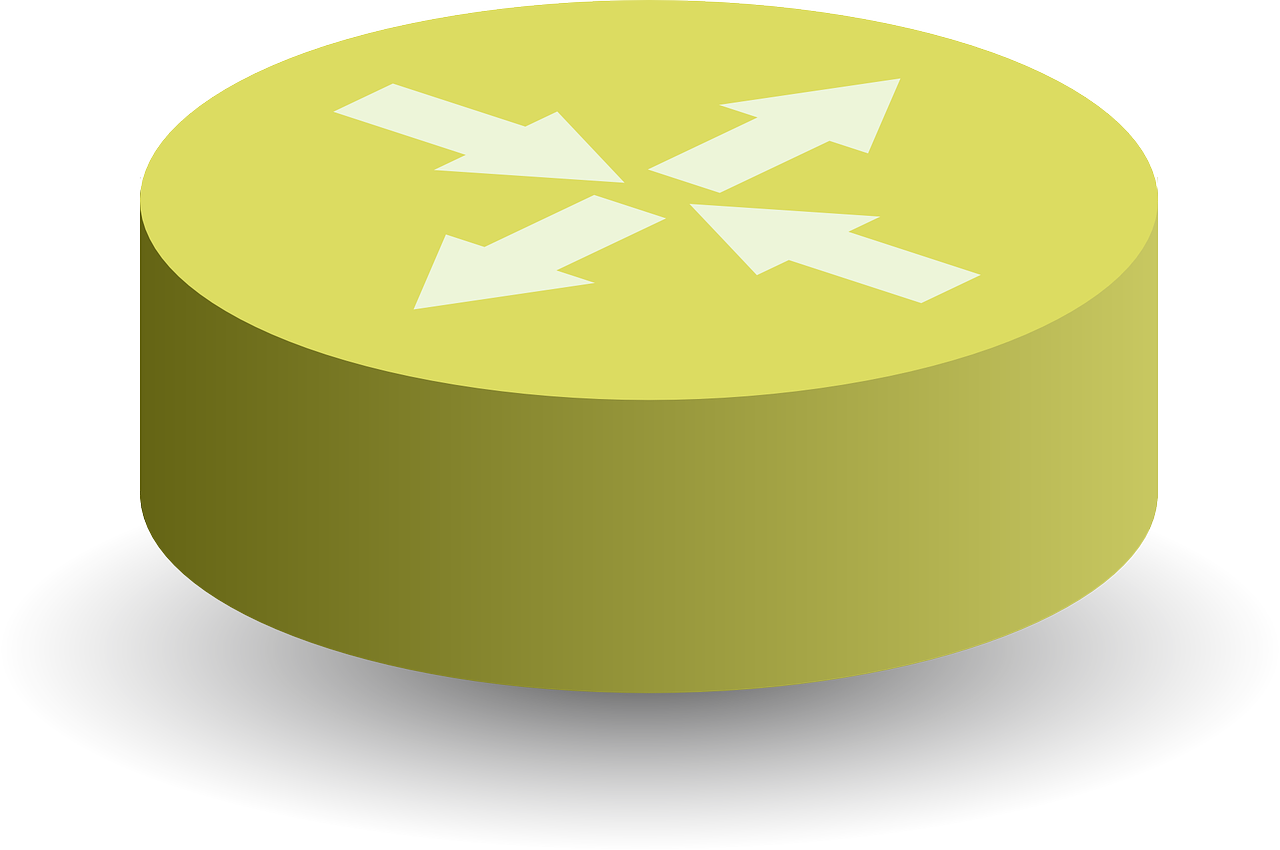
\includegraphics[width=52.5pt,height=52.5pt]{figures/router-158644_1280.png}};
%Image [id:dp370061399936939] 
\draw (412.5,120.5) node  {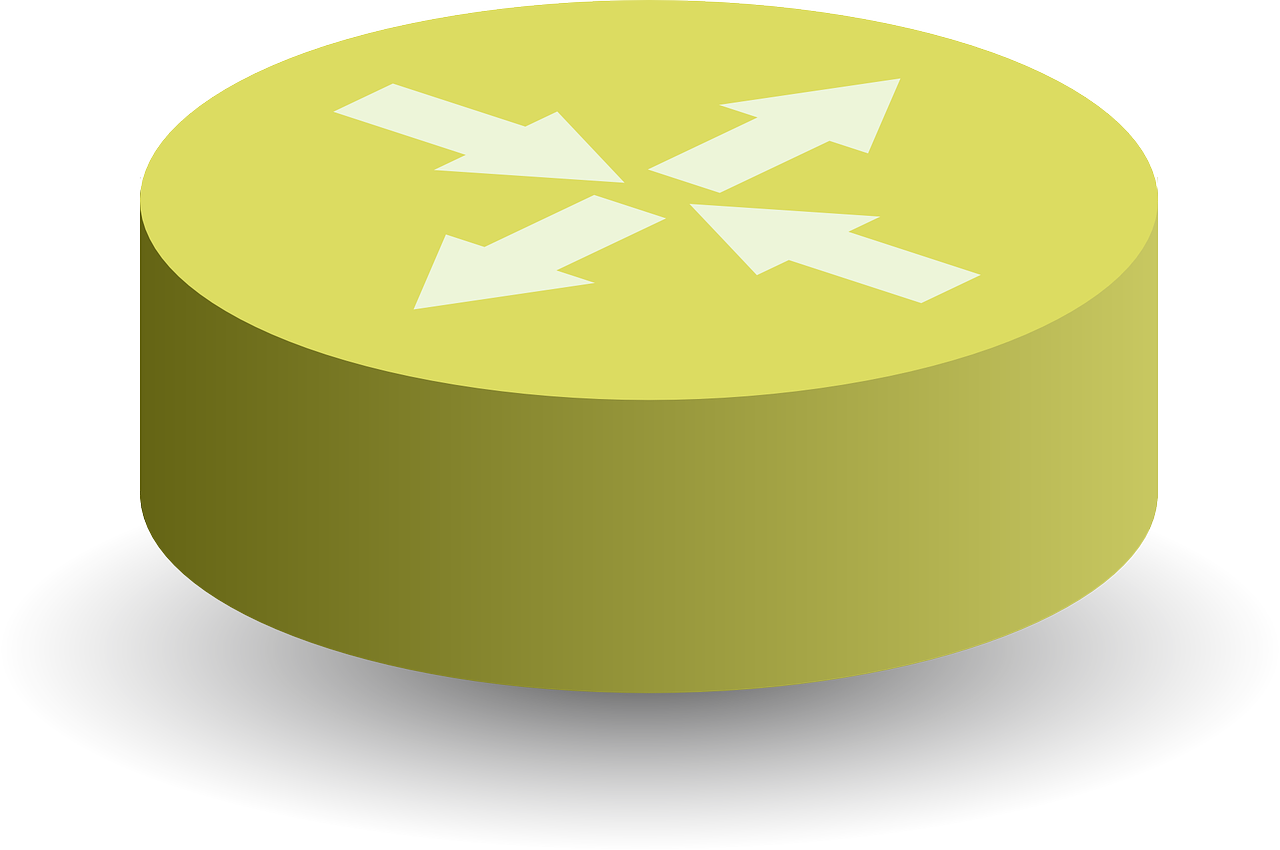
\includegraphics[width=52.5pt,height=52.5pt]{figures/router-158644_1280.png}};
%Image [id:dp4531875445870204] 
\draw (502,120.5) node  {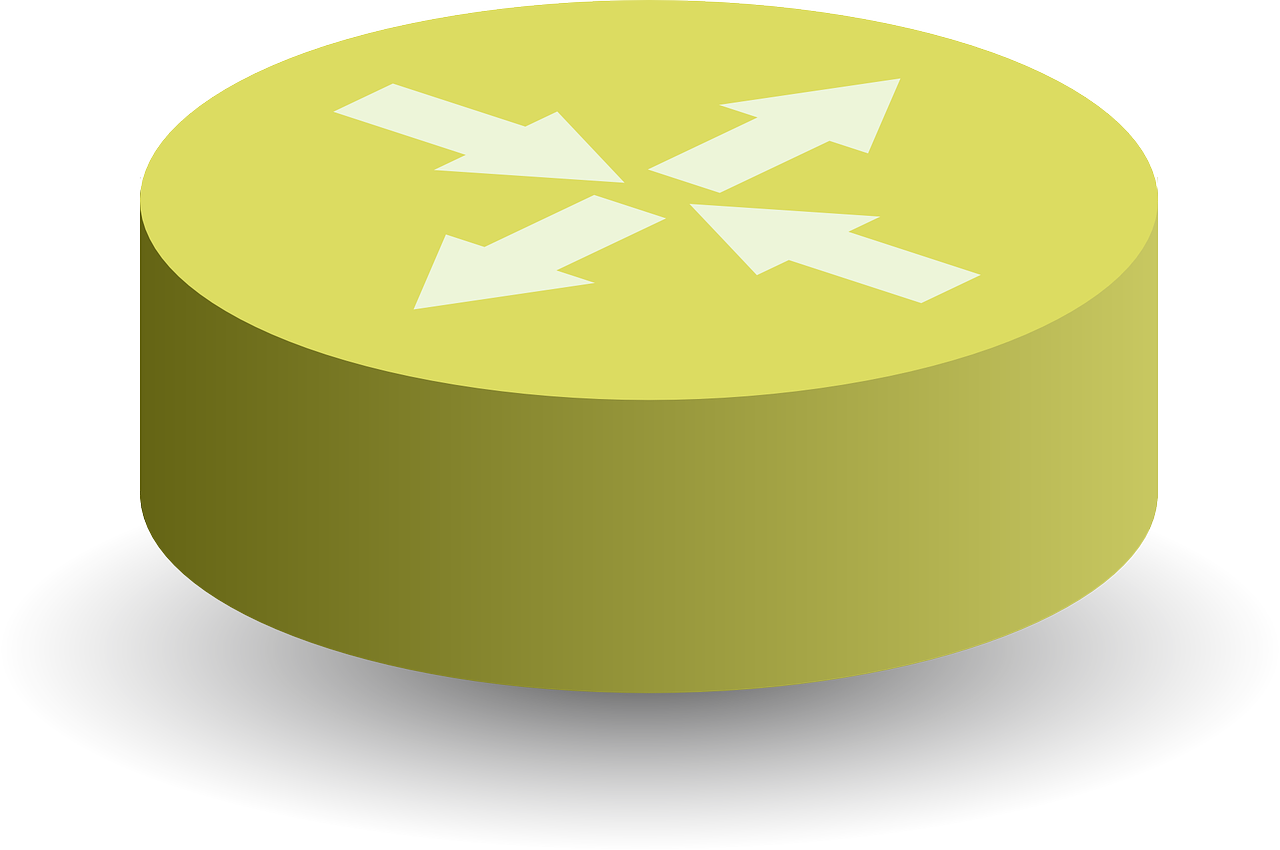
\includegraphics[width=52.5pt,height=52.5pt]{figures/router-158644_1280.png}};

%Rounded Rect [id:dp47820441471440045] 
\draw  [fill={rgb, 255:red, 255; green, 248; blue, 177 }  ,fill opacity=1 ] (46,95.27) .. controls (46,75.05) and (62.39,58.67) .. (82.6,58.67) -- (198.4,58.67) .. controls (218.61,58.67) and (235,75.05) .. (235,95.27) -- (235,205.07) .. controls (235,225.28) and (218.61,241.67) .. (198.4,241.67) -- (82.6,241.67) .. controls (62.39,241.67) and (46,225.28) .. (46,205.07) -- cycle ;
%Straight Lines [id:da6763053778165418] 
\draw    (76,150.67) -- (186,104.67) ;


%Image [id:dp8140812900187272] 
\draw (81,154.5) node  {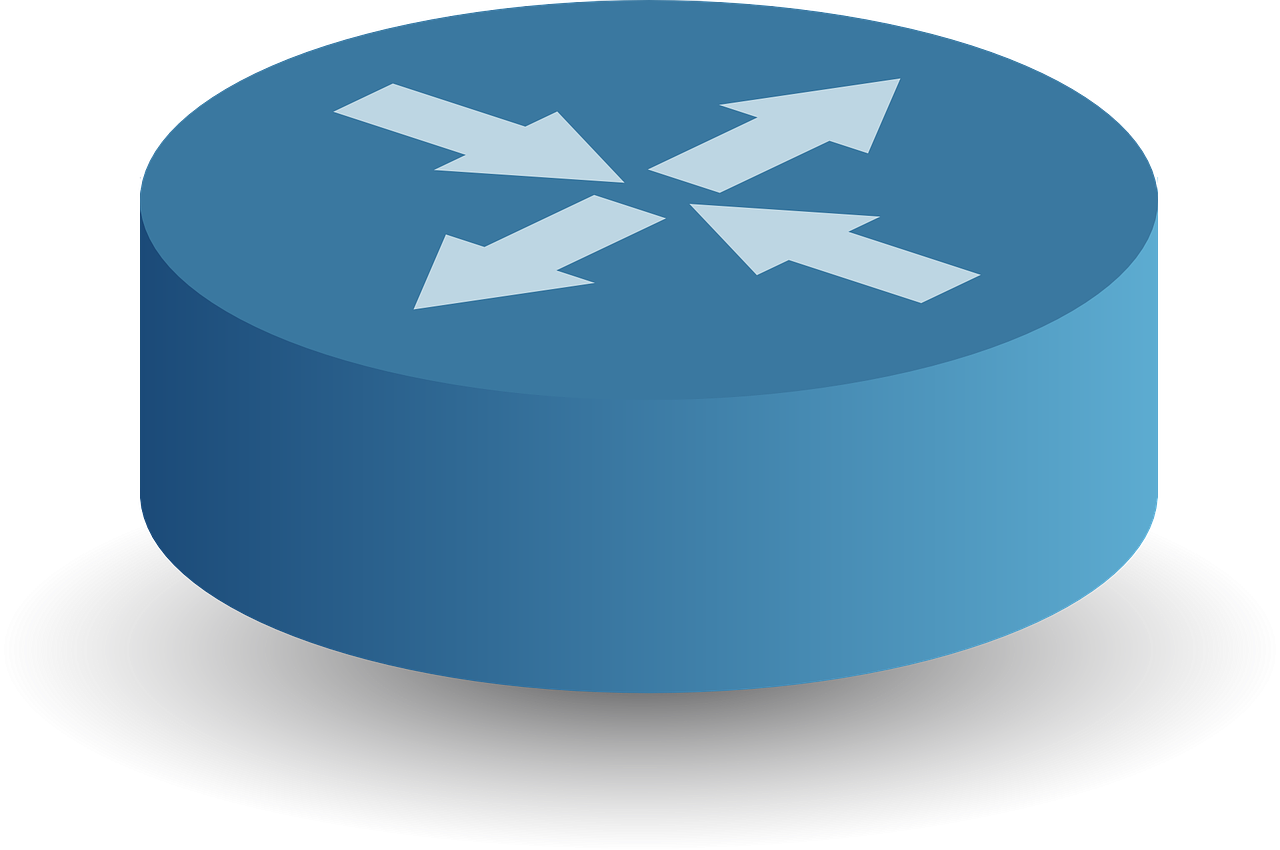
\includegraphics[width=52.5pt,height=52.5pt]{figures/router-29825_1280.png}};
%Image [id:dp7802067738931798] 
\draw (185,100.5) node  {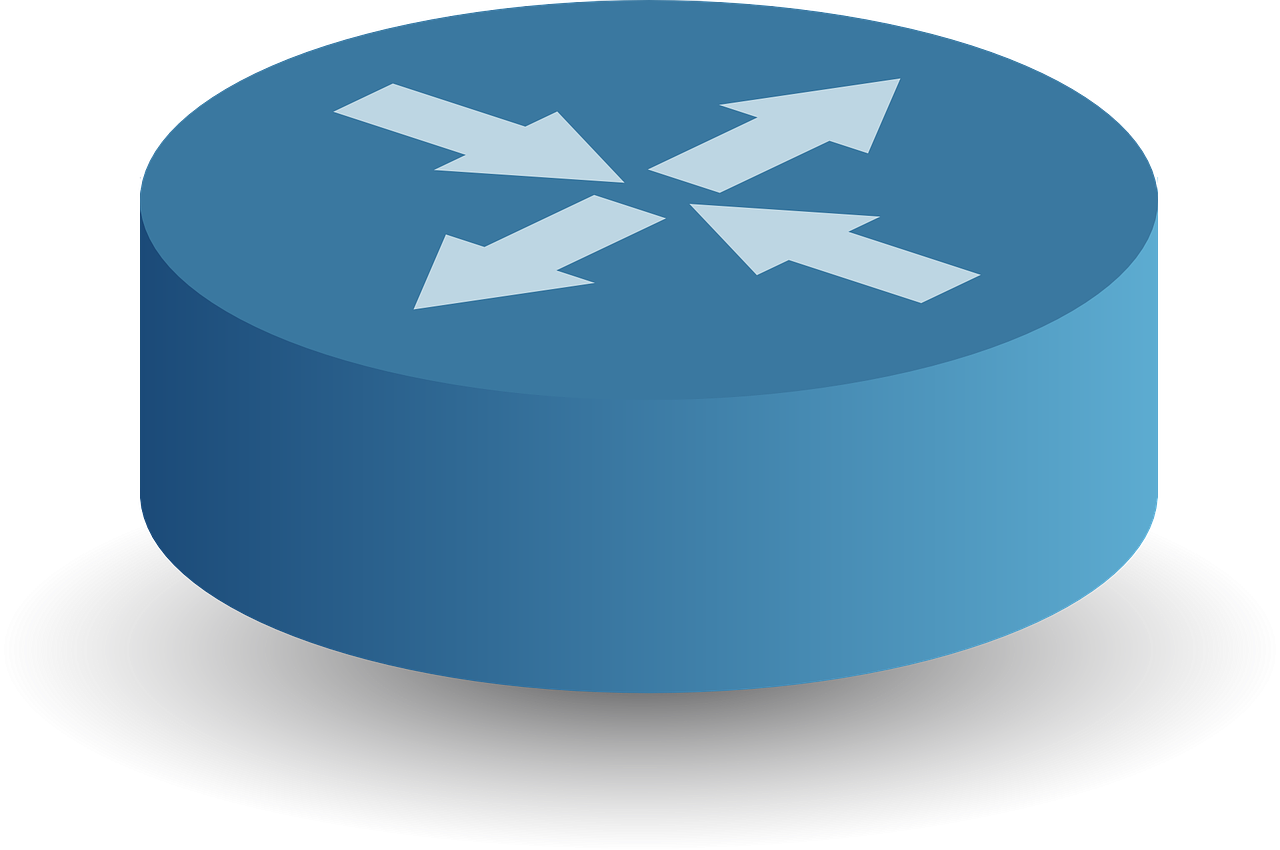
\includegraphics[width=52.5pt,height=52.5pt]{figures/router-29825_1280.png}};

%Straight Lines [id:da4951165105339822] 
\draw    (101,170.17) -- (158,195.67) ;


%Image [id:dp7416941722348419] 
\draw (156,208.5) node  {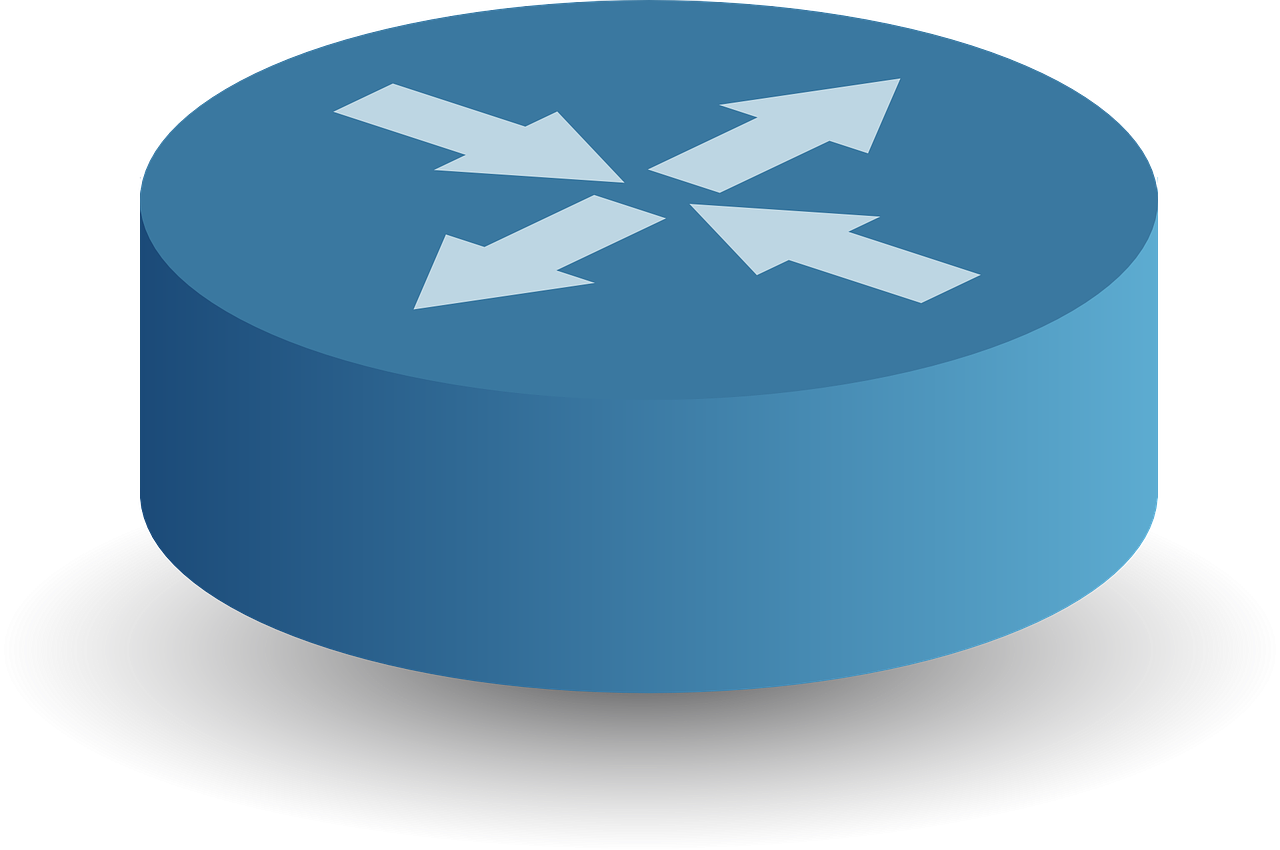
\includegraphics[width=52.5pt,height=52.5pt]{figures/router-29825_1280.png}};

%Rounded Rect [id:dp24159584532295242] 
\draw  [fill={rgb, 255:red, 184; green, 233; blue, 134 }  ,fill opacity=1 ] (27,297.47) .. controls (27,282.11) and (39.45,269.67) .. (54.8,269.67) -- (602.2,269.67) .. controls (617.55,269.67) and (630,282.11) .. (630,297.47) -- (630,380.87) .. controls (630,396.22) and (617.55,408.67) .. (602.2,408.67) -- (54.8,408.67) .. controls (39.45,408.67) and (27,396.22) .. (27,380.87) -- cycle ;
%Straight Lines [id:da4431598038778879] 
\draw    (99,327.67) -- (234,300.67) ;


%Straight Lines [id:da13869241806959443] 
\draw    (100,342.67) -- (191,365.67) ;


%Straight Lines [id:da638319369024069] 
\draw    (194,372.67) -- (388,325.67) ;


%Straight Lines [id:da0876024287705166] 
\draw    (234,300.67) -- (378,309.67) ;


%Straight Lines [id:da03053485372734699] 
\draw    (404,319.67) -- (522,306.67) ;


%Straight Lines [id:da8278064324522899] 
\draw    (395,339.67) -- (497,375.67) ;


%Image [id:dp619468693007916] 
\draw (90,342.5) node  {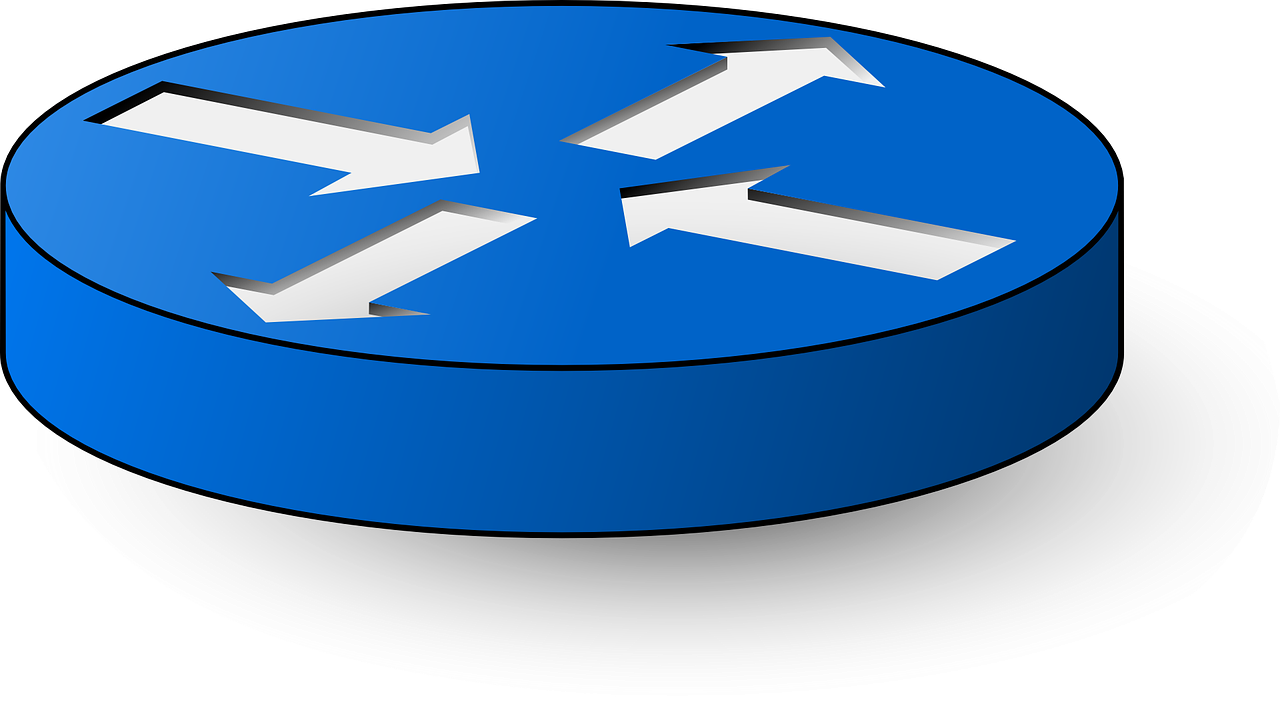
\includegraphics[width=52.5pt,height=52.5pt]{figures/router-30140_1280.png}};
%Image [id:dp8001089418713573] 
\draw (180,373.5) node  {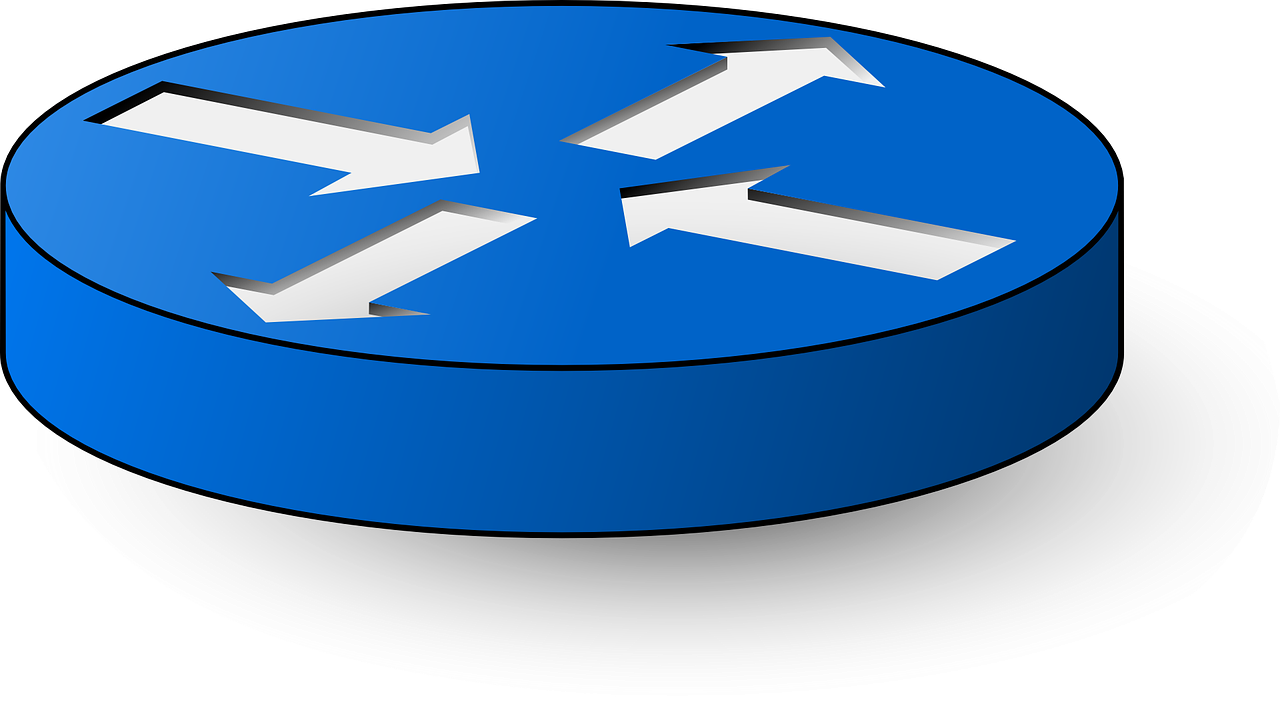
\includegraphics[width=52.5pt,height=52.5pt]{figures/router-30140_1280.png}};
%Image [id:dp9285996053263255] 
\draw (220,310.5) node  {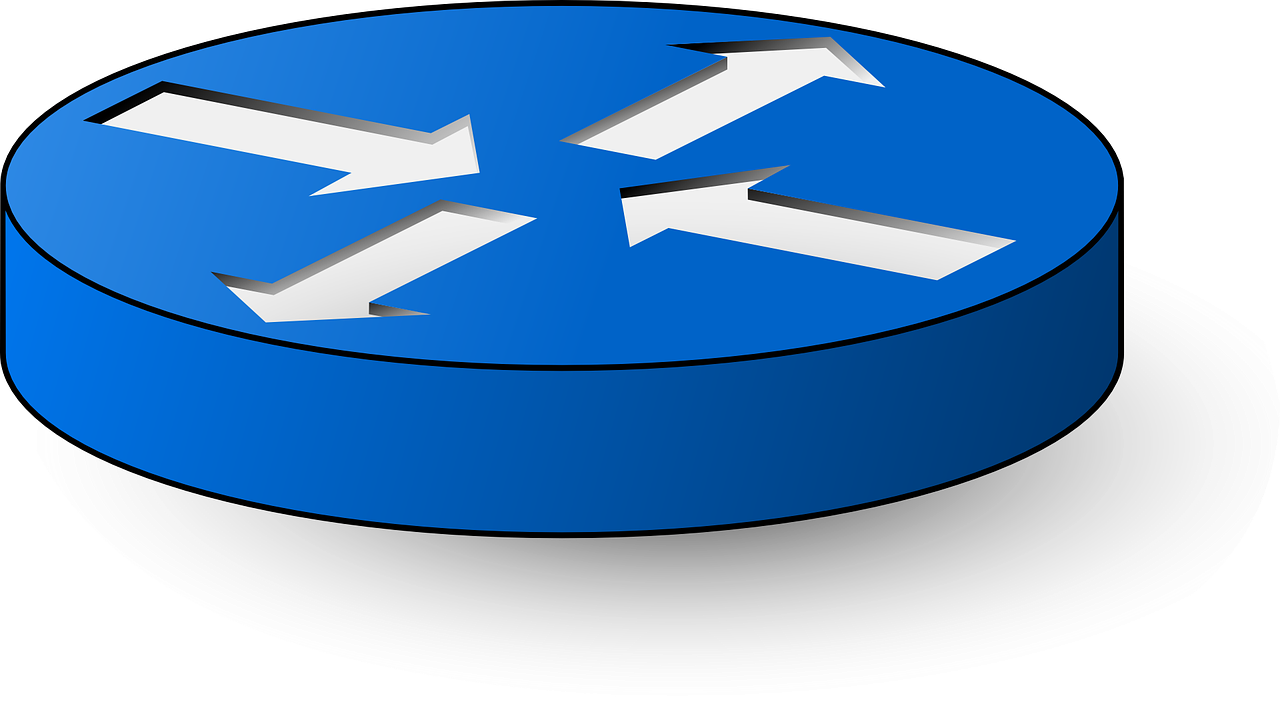
\includegraphics[width=52.5pt,height=52.5pt]{figures/router-30140_1280.png}};
%Image [id:dp3146785253004203] 
\draw (406,324.5) node  {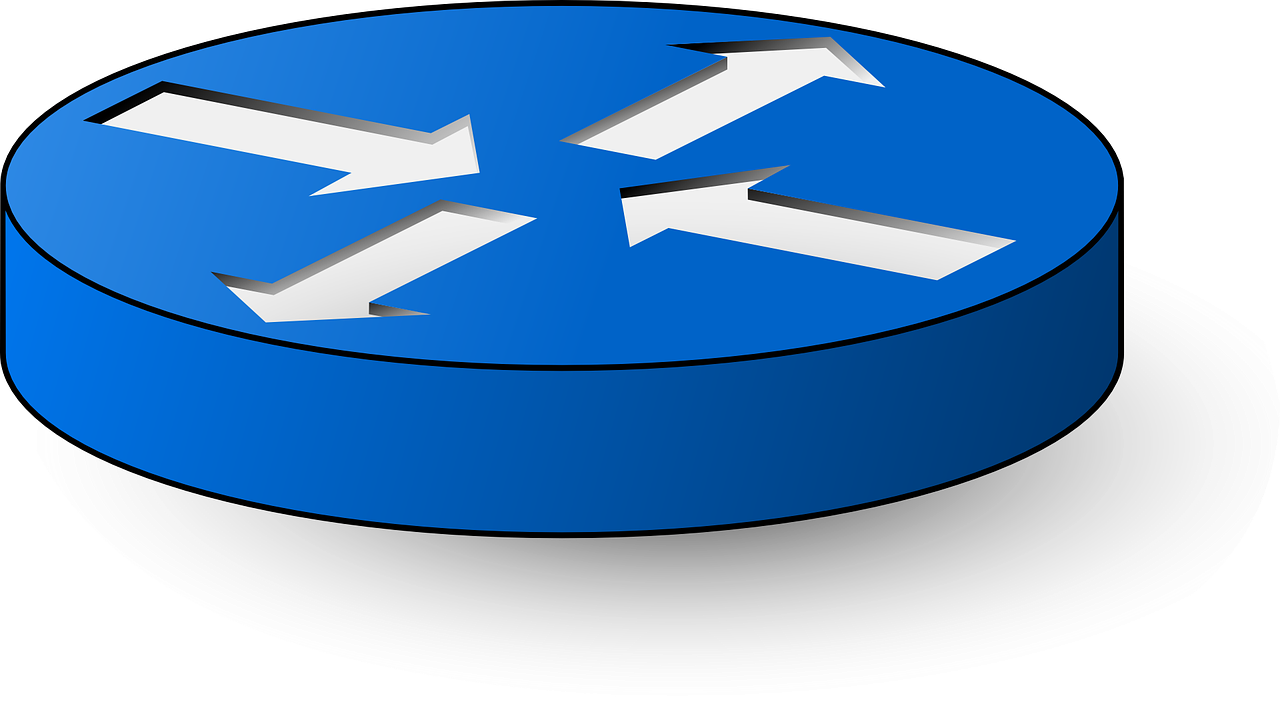
\includegraphics[width=52.5pt,height=52.5pt]{figures/router-30140_1280.png}};
%Image [id:dp3289010965024106] 
\draw (535,313.5) node  {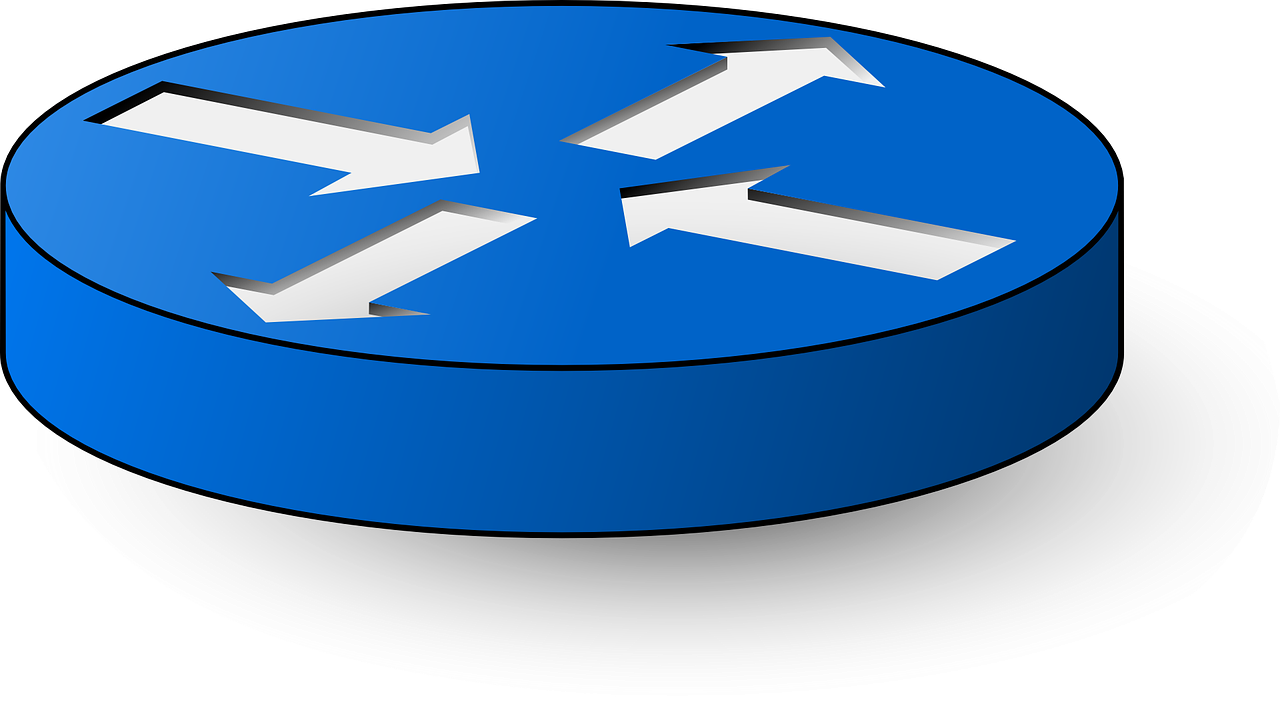
\includegraphics[width=52.5pt,height=52.5pt]{figures/router-30140_1280.png}};
%Image [id:dp13463717449619406] 
\draw (535,386.5) node  {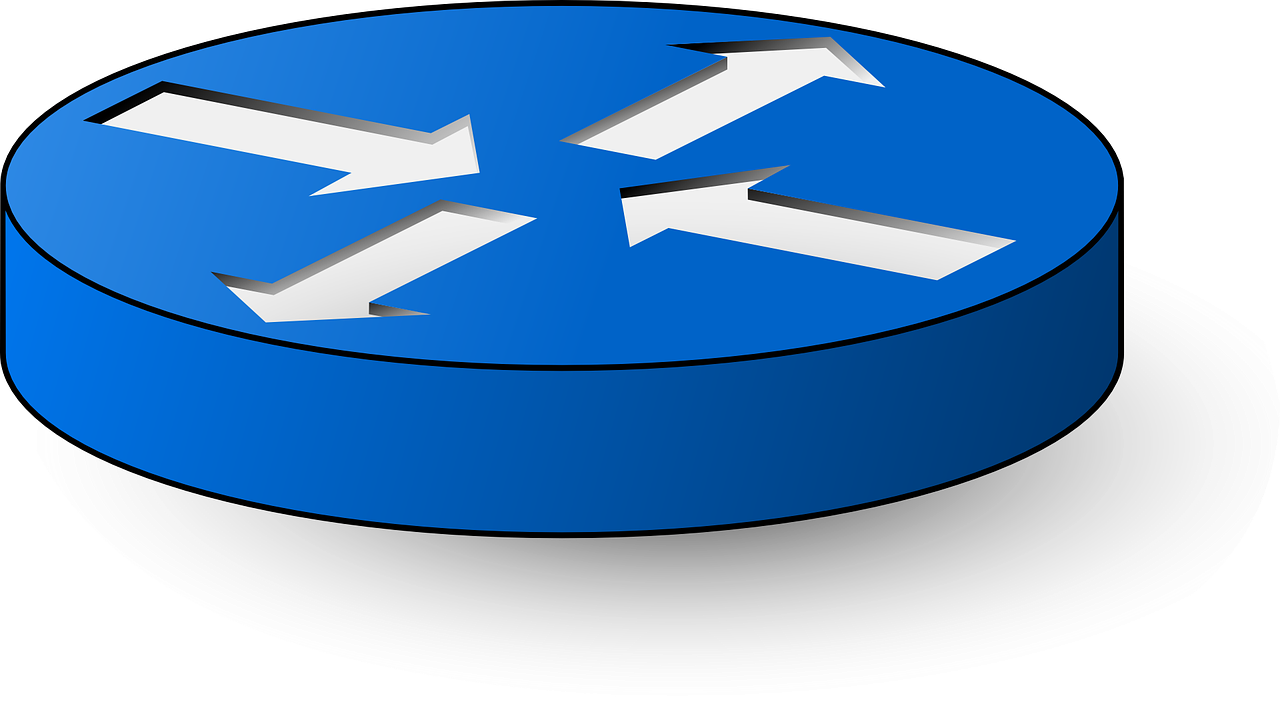
\includegraphics[width=52.5pt,height=52.5pt]{figures/router-30140_1280.png}};
%Straight Lines [id:da2794186668497024] 
\draw [line width=1.5]  [dash pattern={on 1.69pt off 2.76pt}]  (83,177.17) -- (82,307.97) ;


%Straight Lines [id:da3468403679668073] 
\draw [line width=1.5]  [dash pattern={on 1.69pt off 2.76pt}]  (158,228.17) -- (160,341.97) ;


%Straight Lines [id:da6099923036688548] 
\draw [line width=1.5]  [dash pattern={on 1.69pt off 2.76pt}]  (196,123.17) -- (197.2,280.27) ;


%Straight Lines [id:da9880025849572002] 
\draw [line width=1.5]  [dash pattern={on 1.69pt off 2.76pt}]  (318,140.17) -- (235.6,279.47) ;


%Straight Lines [id:da6145453947319308] 
\draw [line width=1.5]  [dash pattern={on 1.69pt off 2.76pt}]  (516,141.17) -- (515.6,283.07) ;


%Straight Lines [id:da41673177695849406] 
\draw [line width=1.5]  [dash pattern={on 1.69pt off 2.76pt}]  (413,143.17) -- (410.4,290.27) ;



% Text Node
\draw (105,397.5) node [scale=0.9] [align=left] {Physical Infrastructure};
% Text Node
\draw (89,74.5) node  [align=left] {{\small vSDN1}};
% Text Node
\draw (327,70.5) node [scale=0.9] [align=left] {{\small vSDN2}};


\end{tikzpicture}}


\caption{Principle of Virtual Network Embedding.}
\label{fig:VNE}
\end{figure}
